\chapter{Intégration SIEM avec Wazuh}

\section{Présentation de Wazuh}

Wazuh est une plateforme SIEM open-source (fork d'OSSEC) offrant une analyse en temps réel des événements de sécurité, une détection d'intrusion basée sur des règles et une conformité réglementaire (PCI-DSS, GDPR). Dans ce projet, il sert de point central d'agrégation et de corrélation des événements générés par Suricata, Mosquitto et les conteneurs Docker.

\section{Déploiement de Wazuh OVA}

\subsection{Choix du mode de déploiement}

Après avoir évalué l'option Docker Compose (qui présentait des incompatibilités avec l'environnement GNS3), le déploiement final retenu est l'OVA officielle Wazuh v4.7 sur VMware Workstation Pro.

\textbf{Configuration de la VM Wazuh :}
\begin{itemize}
  \item \textbf{Adresse IP} : 192.168.30.128
  \item \textbf{RAM} : 8 GB
  \item \textbf{vCPU} : 4
  \item \textbf{Stockage} : 50 GB
  \item \textbf{Dashboard} : \texttt{https://192.168.30.128}
  \item \textbf{Credentials} : \texttt{admin} / \texttt{*Admin1234!}
\end{itemize}

\subsection{Architecture Wazuh}

La solution Wazuh déployée comprend une architecture single-node :
\begin{itemize}
  \item \textbf{Wazuh Manager} : Moteur de règles, corrélation, agrégation.
  \item \textbf{Wazuh Indexer} : Stockage et indexation (OpenSearch).
  \item \textbf{Wazuh Dashboard} : Interface de visualisation (OpenSearch Dashboards).
\end{itemize}

\section{Configuration de l'ingestion Suricata}

\subsection{Configuration du logcollector}

L'agent Wazuh Manager est configuré pour surveiller le fichier EVE JSON de Suricata en mode \texttt{tail} :

\begin{lstlisting}[language=xml, caption=Configuration ossec.conf pour l'ingestion Suricata]
<ossec_config>
  <localfile>
    <log_format>json</log_format>
    <location>/var/log/suricata/eve.json</location>
    <query>
      $.event_type == "alert"
    </query>
  </localfile>
</ossec_config>
\end{lstlisting}

\subsection{Règles de corrélation personnalisées}

Quatre règles custom (IDs 100200-100203) ont été créées dans \texttt{/var/ossec/etc/rules/local\_rules.xml} pour élever le niveau de sévérité des alertes Suricata :

\begin{lstlisting}[language=xml, caption=Règles Wazuh personnalisées pour les alertes IoT]
<group name="suricata,iot,">
  <!-- Alerte TLS sur port MQTT -->
  <rule id="100200" level="3">
    <if_group>suricata</if_group>
    <field name="dest_port">8883</field>
    <description>Suricata: TLS MQTT traffic alert</description>
    <group>tls,mqtt,</group>
  </rule>

  <!-- Alerte générique Suricata -->
  <rule id="100201" level="6">
    <if_group>suricata</if_group>
    <field name="alert.severity">^[123]$</field>
    <description>Suricata: $(alert.signature)</description>
    <group>ids,</group>
  </rule>

  <!-- Attaque DoS IoT -->
  <rule id="100202" level="10">
    <if_sid>100201</if_sid>
    <field name="alert.category">Denial of Service</field>
    <description>IoT DoS Attack detected: $(alert.signature)</description>
    <group>dos,attack,</group>
  </rule>

  <!-- Volume élevé d'alertes -->
  <rule id="100203" level="8" frequency="10" timeframe="60">
    <if_matched_sid>100201</if_matched_sid>
    <same_field>src_ip</same_field>
    <description>High volume of IDS alerts from $(src_ip)</description>
    <group>correlation,</group>
  </rule>
</group>
\end{lstlisting}

\section{Visualisation dans le dashboard}

\subsection{Dashboard Wazuh — résultats}

Les 51 alertes Suricata ont été correctement ingérées et indexées dans Wazuh. Elles sont visibles via le filtre \texttt{rule.groups: suricata} dans l'interface de découverte.

\begin{figure}[H]
  \centering
  % 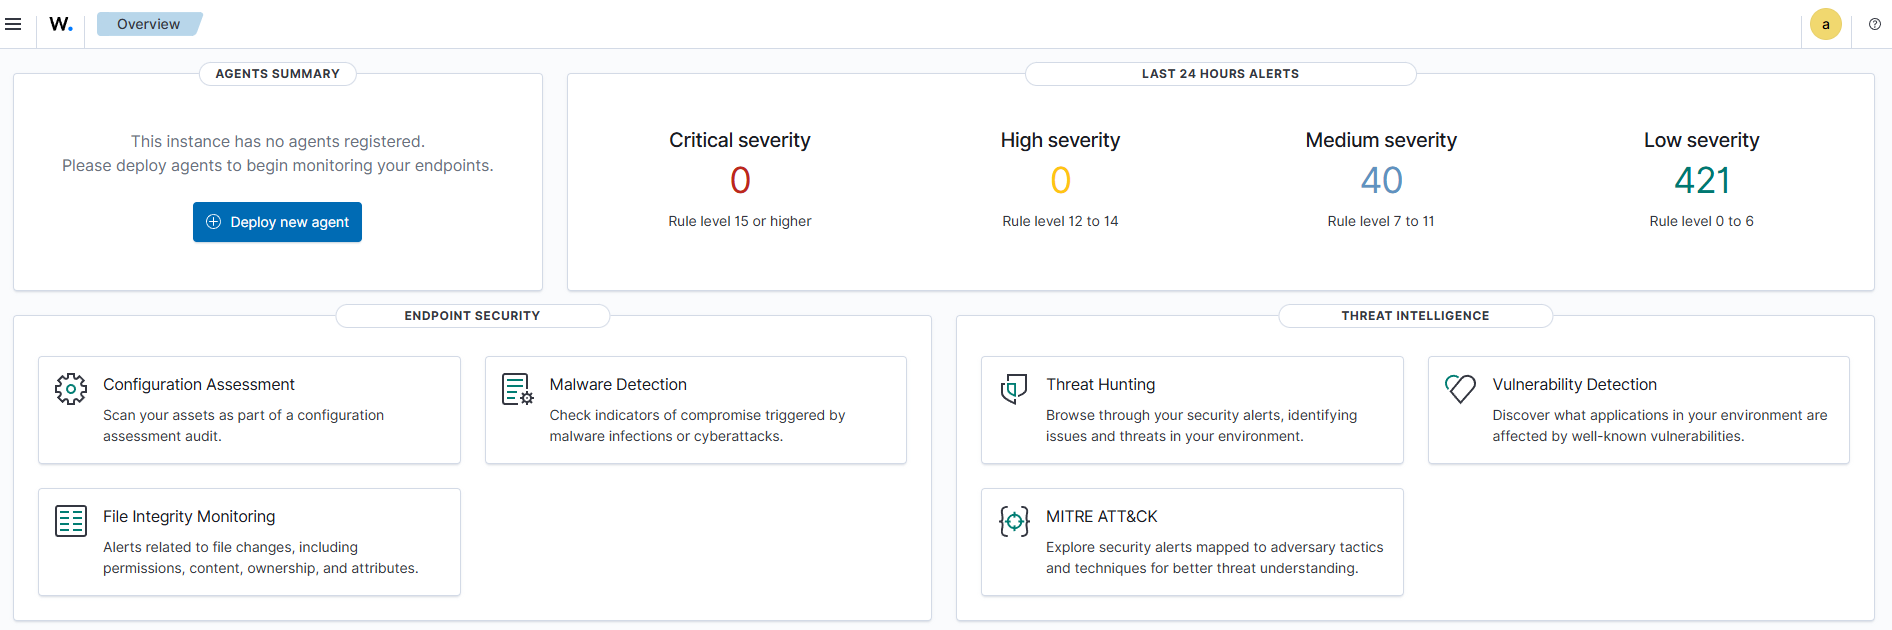
\includegraphics[width=\textwidth]{figures/wazuh-dashboard.png}
  \fbox{\parbox{0.9\textwidth}{\centering\vspace{2cm}\textit{[Figure : Dashboard Wazuh avec alertes Suricata — capture d'écran à insérer]}\vspace{2cm}}}
  \caption{Dashboard Wazuh affichant les alertes IoT/MQTT}
  \label{fig:wazuh_dashboard}
\end{figure}

\subsection{Distribution des alertes par niveau}

\begin{table}[H]
\centering
\caption{Distribution des alertes par niveau de sévérité Wazuh}
\label{tab:wazuh_levels}
\begin{tabular}{lll}
\toprule
\textbf{Niveau} & \textbf{Règle} & \textbf{Alertes} \\
\midrule
3 (Low) & 100200 — TLS MQTT & 18 \\
6 (Medium) & 100201 — Generic Suricata & 20 \\
8 (High) & 100203 — High volume & 9 \\
10 (Critical) & 100202 — DoS Attack & 4 \\
\bottomrule
\end{tabular}
\end{table}

\begin{tcolorbox}[colback=green!5, colframe=green!50!black, title=Résultats Wazuh SIEM]
\begin{itemize}
  \item \textbf{51 alertes Suricata} ingérées et indexées avec succès.
  \item \textbf{4 alertes critiques} (niveau 10) pour les attaques DoS — escalade correctement appliquée.
  \item Corrélation multi-sources opérationnelle (Suricata + logs système).
  \item Dashboard visible à \texttt{https://192.168.30.128} avec visualisations temps-réel.
\end{itemize}
\end{tcolorbox}
